\documentclass[12pt,a4paper,titlepage]{article}
\usepackage[utf8]{inputenc}
\usepackage[T1]{fontenc}
\usepackage[top=3cm, bottom=3cm, left=2cm, right=2cm]{geometry}
\usepackage{textcomp}
\usepackage{amsmath}
\usepackage{amsfonts}
\usepackage{amssymb}
\usepackage{amsthm}
\usepackage{titlesec}
\usepackage{fancyhdr}
\usepackage{lastpage}
\usepackage{fix-cm}
\usepackage{graphicx}
\usepackage{hyperref}
\usepackage{xcolor}
\usepackage{mdwlist}
\usepackage{listings}
\usepackage{float}
\usepackage{wrapfig}
\usepackage{datetime}
\usepackage[perpage,para,bottom,marginal]{footmisc}
\usepackage{listings}
\usepackage{caption}
\usepackage{enumitem}
\usepackage{multicol}
\usepackage[cmtip,all]{xy}
\newdateformat{dmny}{\monthname[\THEMONTH] \THEYEAR}
\newdateformat{dyo}{\THEYEAR}
\setlength{\headheight}{30pt}
\pagestyle{fancy}

\author{Nicolas Hafner}
\lhead{Nicolas Hafner}
\title{Analysis II}
\chead{Analysis II}
\rhead{Zürich, \dmny\today}
\cfoot{\thepage\ / \pageref{LastPage}}
\lfoot{\copyright \dyo\today TymoonNET/NexT}
\date{\d_mny\today}

\newcommand{\longsquiggly}{\xymatrix{{}\ar@{~>}[r]&{}}}

\begin{document}	
\begin{center}{\bfseries\Huge Analysis II - 2014.02.17}\end{center}
\section*{Differentialgleichungen}
\emph{Gewöhnliche} Differentialgleichungen(DGL) sind solche in denen nur eine Variable vorkommt. D.h. Gleichungen von Funktionen einer reellen Variablen. Beispiel: $y=y(x),\; F(x,y..y^{(k)})=0$ ist eine \emph{implizite} DGL der Ordnung $k$. Variante: $y^{(k)}=G(x,y..y^{(k-1)})$ ist eine \emph{explizite} DGL der Ordnung $k$. \\

\textit{Bsp}: Eine DGL der Ordnung 1, mit $G:U\to\mathbb{R},\; U\in\mathbb{R}^2$ bildet ein Vektorfeld $K$. Der Graph einer Lösung ist überall tangential zu $K$. \\

\textit{Bsp}: Eine DGL der Ordnung 2, mit $U\subset\mathbb{R}^3$. Die Lösung der DGL ist eine diff'bare Funktion $y$ auf einem Intervall, die die Gleichung löst. \\

\emph{Anfangswertproblem}: Gegeben sei eine DGL mit $G:U\to\mathbb{R}$, mit Anfangswert $(x_0,y_0..y^{(k-1)}_0)\in U$. Ein \emph{Randwertproblem} andererseits wäre eine DGL mit Bedingungen der Form $y^{(l_i)}(t_i)=y_i$ für gegebene $i,l_i,t_i$.

\section*{Existenz und Eindeutigkeit}
\textit{Def}: Eine Funktion $f:X\to Y$ heisst (global) Lipschitzstetig falls
$$\exists c>0:\forall x,x'\in X:|f(x)-f(x')|\leq c\cdot|x-x'|$$
Eine Funktion $f:X\to Y$ heisst lokal Lipschitzstetig, falls $X$ durch offene Mengen $U_i$ überdeckt werden kann, so dass $f|U_i$ lipschitzstetig ist. Für $X=\mathbb{R}^n$ heisst das, dass $c$ von $|x|+|x'|$ abhängen darf. \\

\textit{Fakt}: \begin{enumerate}[label=(\alph*)]
\item Jede differenzierbare Funktion mit stetiger Ableitung ist lokal libschitzstetig.
\item Die Grundrechenarten sind lokal lipschitzstetig.
\item Jede Komposition von lokal lipschitzstetigen Funktionen ist lokal lipschitzstetig.
\item Eine vektorwertige Funktion ist lokal lipschitzstetig $\Leftrightarrow$ jede Komponenten der Funtion ist es.
\end{enumerate}

\textit{Bsp}: $\mathbb{R}^n\to\mathbb{R},\;x\mapsto|x|$ ist lipschitzstetig. (Dreiceksungleichung). \\

\textit{Bsp}: $\mathbb{R}^2\to\mathbb{R},\;(x,y)\mapsto x\cdot y$ ist lokal ipschitzstetig aber nicht global.

\section*{Existenz- und Eindeutigkeitssatz}
Sei $U\subset\mathbb{R}^{n+1}$ offen und $F:U\to\mathbb{R}$ lokal lipschitzstetig. Sei $(x_0,y_o..y_o^{(n-1)})\in U$ ein Anfangswert. Dann gilt: \begin{enumerate}[label=(\alph*)]
\item Die DGL $y^{(n)}=F(x,y..y^{(n-1)})$ mit dem AW $y(x_0)=y_0,..y^{(n-1)}(x_0)=y_0^{(k-1)}$ bildet eine Lösung $y:(x-\epsilon_1,x+\epsilon_2)\to\mathbb{R}$ mit $\epsilon_1,\epsilon_2>0$.
\item Je zwei solche Lösungen $y$ auf $(x_0-\epsilon_1,x_0+\epsilon_2)$ bzw $\widetilde{y}$ auf $(x_0-\widetilde{\epsilon_1},x_0+\widetilde{\epsilon_2})$ stimmen auf dem Durchschnitt der Intervalle überein.
\item Es existiert eine eindutige ``maximale'' Lösung, d.h. eine mit maximalem, offenem Definitionsintervall $]x_1,x_2[$.
\item Diese max. Lösung verlässt jede kompakte Teilmenge $K\subset U$, d.h. $\exists\xi<x_2:\forall x\in]\xi,x_1[:(y,y(x)..y^{(k-1)}(x))\notin K$. D.h. sie geht nach Unendlich oder zum Rand von $U$.
\end{enumerate}

\section*{Orthogonaltrajektion}
\textit{Bsp}: $y'=\frac{y}{x}$ auf $(\mathbb{R}^{>0})^2$. \\
\begin{figure}[H]\centering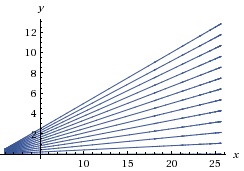
\includegraphics{WolframAlpha--y__y_x__Sample_solution_family__2014_02_17_0239.png}\end{figure}
Durch Raten $\longsquiggly\forall\lambda>0:\; y:=\lambda x$ ist Lösung. $\mathbb{R}^{>0}\to\mathbb{R}^{>0}$ ist maximal. Durch $(x_0,y_0)\in U$ geht die Lösung $y:=\frac{y_0}{x_0}\cdot x$. Also sind dies \emph{alle} max. Lösungen. \\

\textit{Bsp}: Orthogonal dazu: $y'=-\frac{x}{y}$ \\
\begin{figure}[H]\centering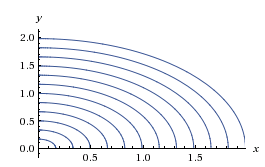
\includegraphics{WolframAlpha--y-xy--2014-02-17_0244.png}\end{figure}
Rate: $y=\sqrt{r^2-x^2}$, $r>c$. $]0,r[\to\mathbb{R}$. $\frac{dy}{dx}=\frac{1}{2\sqrt{r^2-x^2}}\cdot(-2x) = \frac{-x}{y}$. Ex+Eind.Satz $\Rightarrow$ Dies sind alle max. Lösungen. \\

\textit{Bsp}: $y'=y^2$ auf $\mathbb{R^2}=U$. \\
\begin{figure}[H]\centering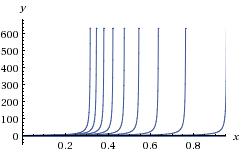
\includegraphics{WolframAlpha--y__y_2__Sample_solution_family__2014_02_17_0253.png}\end{figure}
$\frac{dx}{dy}=y^2$. $y$ invertiert? \longsquiggly $\frac{dx}{dy}=\frac{1}{y^2} \Rightarrow x(y)=\int\frac{1}{y^2}dy=c-\frac{1}{y}=\frac{cy-1}{y}=x \Rightarrow cy-1=yx \Rightarrow cy-yx=1 \Rightarrow y=\frac{1}{c-x}$. Also \emph{setze}: $y:=\frac{1}{c-x}$ für $c\in\mathbb{R}$ fest. \longsquiggly $y'=\frac{-1\cdot(c-x)'}{(c-x)^2}=\frac{1}{(c-x)^2}=y^2$
\begin{enumerate}
\item $y:]c,\infty[\to\mathbb{R},\; x\mapsto\frac{1}{c-x}$
\item $y:]-\infty,\infty[\to\mathbb{R},\; x\mapsto\frac{1}{c-x}$
\item $y:\mathbb{R}\to\mathbb{R},\; x\mapsto 0$
\end{enumerate}
\end{document}